%%%%%%%%%%%%%%%%%%%%%%%%%%%%%%%%%%%%%%%%%
% University Assignment Title Page 
% LaTeX Template
% Version 1.0 (27/12/12)
%
% This template has been downloaded from:
% http://www.LaTeXTemplates.com
%
% Original author:
% WikiBooks (http://en.wikibooks.org/wiki/LaTeX/Title_Creation)
%
% License:
% CC BY-NC-SA 3.0 (http://creativecommons.org/licenses/by-nc-sa/3.0/)
% 
% Instructions for using this template:
% This title page is capable of being compiled as is. This is not useful for 
% including it in another document. To do this, you have two options: 
%
% 1) Copy/paste everything between \begin{document} and \end{document} 
% starting at \begin{titlepage} and paste this into another LaTeX file where you 
% want your title page.
% OR
% 2) Remove everything outside the \begin{titlepage} and \end{titlepage} and 
% move this file to the same directory as the LaTeX file you wish to add it to. 
% Then add \input{./title_page_1.tex} to your LaTeX file where you want your
% title page.
%
%%%%%%%%%%%%%%%%%%%%%%%%%%%%%%%%%%%%%%%%%
%\title{Title page with logo}
%----------------------------------------------------------------------------------------
%	PACKAGES AND OTHER DOCUMENT CONFIGURATIONS
%----------------------------------------------------------------------------------------

\documentclass[12pt]{article}
\usepackage[italian]{babel}
\usepackage[utf8x]{inputenc}
\usepackage{amsmath}
\usepackage{graphicx}
\usepackage[colorinlistoftodos]{todonotes}
\usepackage{float}
\usepackage{adjustbox}
\usepackage{subcaption} 

\begin{document}

\begin{titlepage}

\newcommand{\HRule}{\rule{\linewidth}{0.5mm}} % Defines a new command for the horizontal lines, change thickness here

\center % Center everything on the page
 
%----------------------------------------------------------------------------------------
%	HEADING SECTIONS
%----------------------------------------------------------------------------------------

\textsc{\LARGE Università degli studi di Milano-Bicocca}\\[1cm] % Name of your university/college
\textsc{\Large Advanced Machine Learning }\\[0.3cm] % Major heading such as course name
\textsc{\large Progetto Finale}\\[0.1cm] % Minor heading such as course title

%----------------------------------------------------------------------------------------
%	TITLE SECTION
%----------------------------------------------------------------------------------------

\HRule \\[0.4cm]
{ \huge \bfseries Classificazione di immagini su un dataset con molte classi simili tra di loro}\\[0.4cm] % Title of your document
\HRule \\[1.5cm]
 
%----------------------------------------------------------------------------------------
%	AUTHOR SECTION
%----------------------------------------------------------------------------------------

\large
\emph{Autori:}\\
Lorenzo Mammana - 807391- l.mammana@campus.unimib.it \\   % Your name
Eric Nisoli - 807147- e.nisoli1@campus.unimib.it   \\[1cm] % Your name

% If you don't want a supervisor, uncomment the two lines below and remove the section above
%\Large \emph{Author:}\\
%John \textsc{Smith}\\[3cm] % Your name

%----------------------------------------------------------------------------------------
%	DATE SECTION
%----------------------------------------------------------------------------------------

{\large \today}\\[2cm] % Date, change the \today to a set date if you want to be precise

%----------------------------------------------------------------------------------------
%	LOGO SECTION
%----------------------------------------------------------------------------------------

\hspace*{0.4cm}
\includegraphics[scale=0.75]{logo.png}\\[1cm] % Include a department/university logo - this will require the graphicx package
 
%----------------------------------------------------------------------------------------

\vfill % Fill the rest of the page with whitespace

\end{titlepage}


\begin{abstract}
Il presente lavoro illustra un approccio supervisionato alla classificazione di immagini su un dataset di piccole dimensioni, ma con un grande numero di classi. In particolare viene mostrato come la combinazione di moderne tecniche di addestramento e i recenti sviluppi nel campo della ricerca di architetture per reti neurali, siano in grado di ottenere delle performance comparabili a quelli ottenuti da modelli molto più complessi presenti in letteratura.
\end{abstract}

\section{Introduzione}
L'obiettivo del progetto è quello di costruire un modello di machine learning per la classificazione di immagini in grado di operare bene su un dataset di piccole dimensioni comprendente un alto numero di classi simili tra di loro.
Come è facilmente intuibile, il problema principale di operare su un dataset di questo tipo è l'overfitting del modello sui dati di training con conseguente fallimento del modello su dati nuovi. Per risolvere questo problema ci siamo concentrati sulla ricerca di modelli, iperparametri e tecniche di generalizzazione che permettessero al modello di essere in grado di operare su un dataset di test molto più ampio di quello utilizzato per l'addestramento.
Il modello utilizzato per questo tipo di analisi è una rete neurale convoluzionale (CNN); questo tipo di modello si è dimostrato negli ultimi anni il migliore nel classificare immagini in moltissimi campi di applicazione.
In particolare viene fatto uso di un modello preaddestrato su immagini simili, ci si aspetta quindi che la classificazione finale buona nonostante i problemi iniziali derivati dal dataset.

\section{Dataset}
Il dataset utilizzato è il \textit{102 Category Flower Dataset} \cite{Nilsback08} creato dai ricercatori del \textit{Visual Geometry Group} di \textit{Oxford}. Il dataset è composto da 8189 immagini RGB di dimensione variabile, ogni immagine contiene uno o più fiori su sfondo neutro ed è etichettata con una singola categoria estratta da un insieme di centodue possibili categorie. Il dataset originale contiene anche i fiori segmentati dallo sfondo (Figura \ref{fig_dataset}), queste immagini possono essere usate ad esempio come ulteriore input per la rete neurale. In questo lavoro non sono state utilizzate principalmente per forzare la rete ad essere più elastica rispetto allo sfondo delle immagini.
E' stata mantenuta la suddivisione del dataset definita nella pubblicazione originale, in particolare si hanno:
\begin{itemize}
\item 1020 immagini nel training set
\item 1020 immagini nel validation set
\item 6149 immagini nel test set
\end{itemize}
Ogni categoria è rappresentata da 10 immagini nel training set e nel validation set, mentre la proporzione di immagini per ogni categoria varia nel test set.
La difficoltà di operare su un dataset di questo tipo è evidente, il numero di immagini è limitato mentre il test set è ampio.
\begin{figure}[H]
\centering	
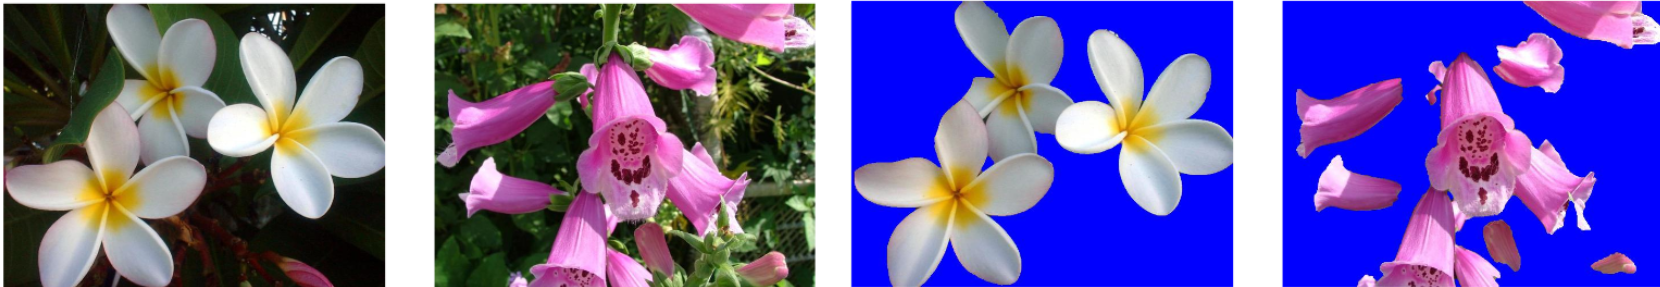
\includegraphics[width=1.0\textwidth]{images/dataset.png} 
\caption{Immagini di training e relativa segmentazione \cite{Nilsback08}}
\label{fig_dataset}
\vspace{-7mm}
\end{figure}


\section{Approccio metodologico}
Per classificare le immagini nelle classi corrette si è deciso di utilizzare una rete neurale convoluzionale. Come è noto addestrare questo tipo di modello richiede un numero di immagini dell'ordine di milioni di elementi, non avendo a disposizione così tante immagini è necessario eseguire la tecnica nota come \textit{finetuning} in cui la CNN viene inizializzata con pesi calcolati su un dataset di milioni di immagini e modificati in accordo con i propri dati disponibili.
Si è deciso quindi di utilizzare reti preaddestrate sul dataset \textit{Imagenet}   \cite{5206848} contenente più di 10 milioni di immagini di cui più di trecentomila rappresentanti fiori.
\subsection{Esperimento baseline}
Considerando il fatto che il numero di immagini di training è limitato, è stato inizialmente deciso di definire un modello baseline non particolarmente complesso. Il modello scelto è una \textit{Resnet18} \cite{he2015deep} preaddestrata su \textit{Imagenet}. Inizialmente si è provato ad utilizzare la rete come estrattore di features per valutare quanto il preaddestramento influisca sulla classificazione finale. 
Le features estratte vengono classificate utilizzando un semplice percettrone multistrato:
\begin{table}[H]
\centering
\caption{Architettura del percettrone}
\begin{tabular}{lll}
\hline
Layer (type)     & Output Shape & Param \# \\ \hline
dense\_1 (Dense) & (None, 256)  & 6422784  \\ \hline
dense\_2 (Dense) & (None, 128)  & 32896    \\ \hline
dense\_3 (Dense) & (None, 102)  & 13158    \\ \hline
\end{tabular}
\label{t_mlp}
\end{table}
L'architettura è stata scelta eseguendo un test automatico di più configurazioni in parallelo.

\subsubsection{Preprocessing e Data augmentation}
Prima di procedere con l'estrazione delle features le immagini vengono normalizzate per avere media nulla e varianza unitaria utilizzando la formula:
\begin{equation}
x' = \frac{x - \overline{x}}{\sigma}
\end{equation}
Dove $ \overline{x} $ e $ \sigma $ rappresentano rispettivamente la media e la varianza calcolate su \textit{Imagenet}.
Questo permette di passare alla rete delle immagini più simili a quelle su cui è stata addestrata ottenendo quindi dei risultati più attendibili.
\subsubsection{Scelta degli iperparametri}
Per addestrare il percettrone sulle features estratte si è deciso di utilizzare il mini-batch stochastic gradient descent (SGD) \cite{kiefer1952}, con dimensione del batch pari a 64 e momentum pari a 0.9.
Essendo il task una classificazione multiclasse e singola label viene utilizzata una cross-entropy categorica come funzione obiettivo da minimizzare.
Il learning rate viene calcolato in accordo con l'algoritmo descritto in "Cyclical Learning Rates for Training Neural Networks" \cite{smith2015cyclical}.
Questo algoritmo prevede che il learning rate oscilli avanti ed indietro in un range prefissato di valori ad ogni iterazione nell'addestramento, questo ha un duplice scopo:
\begin{itemize}
\item Permette all'ottimizzatore di uscire da eventuali punti di sella o da minimi locali che potrebbero bloccarne la corretta convergenza.
\item Riduce il bias introdotto dalla scelta iniziale di un learning rate scorretto.
\end{itemize}
Per calcolare il range su cui far variare il learning rate viene utilizzata una seconda tecnica automatica descritta nello stesso articolo:
\begin{enumerate}
\item Si definiscono un estremo inferiore piccolo ed un estremo superiore grande su cui far variare il learning rate, ad esempio [1e-10, 1e-1].
\item Si addestra la rete per un numero ridotto di epoche partendo dall'estremo inferiore ed incrementando esponenzialmente il learning rate ad ogni batch.
\item Il training continua fino a quando il learning rate non raggiunge l'estremo superiore.
\item Viene plottato un grafico che mostra quando il learning rate è troppo basso o troppo alto.
\end{enumerate} 
L'algoritmo sul percettrone multistrato produce il seguente grafico:
\begin{figure}[ht]
\centering
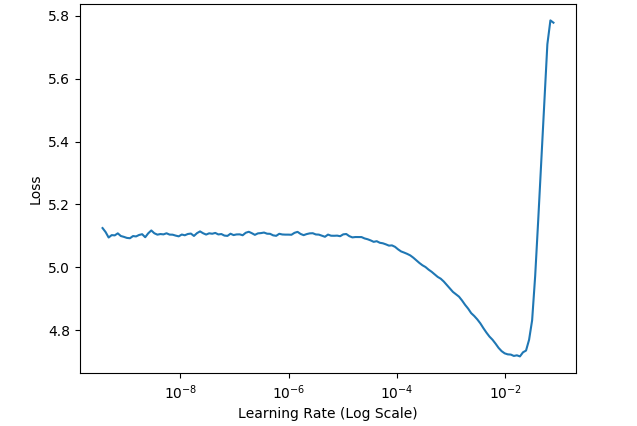
\includegraphics[width=0.8\textwidth]{images/baseline/lrfind_plot.png} 
\caption{Output dell'algoritmo di ricerca del learning rate}
\label{fig_baseline_finder}
\vspace{-15mm}
\end{figure}
\newpage
Dal grafico si vede come la rete cominci ad apprendere circa a partire da 1e-5 e diverga una volta superato 1e-2, questi due valori verranno quindi utilizzati come estremi per l'algoritmo di cyclical learning rate.
Questo algoritmo ha due ulteriori iperparametri, il primo è definito \textit{Step size} ed indica il numero di iterazioni richiesto per passare dal minimo learning rate al massimo, il secondo è il metodo con cui viene modificato il learning rate.
La rete viene addestrata per 50 epoche con diverse coppie di iperparametri; i risultati sono riportati in tabella.
\begin{table}[H]
\centering
\caption{Risultati dei diversi iperparametri sul test set}
\begin{tabular}{|l|l|l|}
\hline
Metodo       & Step size & Test accuracy \\ \hline
Triangular   & 2         & 0.550         \\ \hline
Triangular   & 4         & 0.550         \\ \hline
Triangular   & 6         & 0.558         \\ \hline
Triangular   & 8         & 0.547         \\ \hline
Triangular2  & 2         & 0.510         \\ \hline
Triangular2  & 4         & 0.527         \\ \hline
Triangular2  & 6         & 0.550         \\ \hline
Triangular2  & 8         & 0.533         \\ \hline
Non cyclical & -         & 0.478         \\ \hline
\end{tabular}
\label{t_clr}
\end{table}
L'algoritmo non cyclical utilizza SGD con learning rate iniziale pari a 1e-2 e decay del learning rate di un fattore 0.1 in caso di non decrescita della loss sul set di validazione. E' evidente come l'algoritmo ciclico converga ad una soluzione decisamente migliore e soprattuto lo riesca a fare riducendo al massimo il tempo necessario per cercare il miglior learning rate per la rete.
In tabella vengono mostrati due metodi uno definito \textit{Triangular} e l'altro definito \textit{Triangular2}, la differenza è che il secondo metodo dimezza l'ampiezza dell'intervallo di ricerca del learning rate ad ogni completamento del ciclo, questo è ben visibile plottando la variazione del learning rate nel tempo, come mostrato in figura \ref{fig_lr_tr}.

\begin{figure}[H]
\vspace{-10mm}
\makebox[\linewidth][c]{%
\begin{subfigure}[b]{.6\textwidth}
\centering
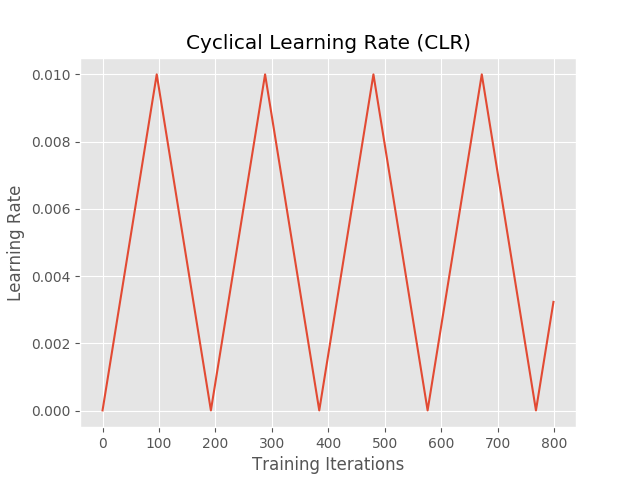
\includegraphics[width=.95\textwidth]{images/baseline/clr_plot_triangular_6.png}
\caption{Triangular}
\end{subfigure}%
\begin{subfigure}[b]{.6\textwidth}
\centering
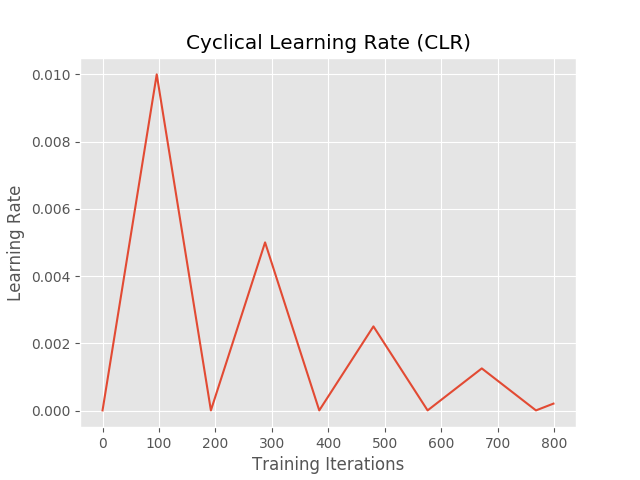
\includegraphics[width=.95\textwidth]{images/baseline/clr_plot_triangular2_6.png}
\caption{Triangular2}
\end{subfigure}%
}\\
\vspace{-7mm}
\caption{Andamento del learning rate con step size 6}
\label{fig_lr_tr}
\vspace{-5mm}
\end{figure}


Da questa prima valutazione si è in grado di notare come il preaddestramento influisca decisamente sulla classificazione del dataset.
\subsection{Esperimento 1 - Finetuning Resnet18}
La sola estrazione delle feature non è ovviamente abbastanza per ottenere delle performance soddisfacenti sul test set, si è proceduto quindi ad eseguire il finetuning dell'intera rete in modo tale da aggiornare i pesi per renderli più compatibili con il nuovo dataset.
Adesso invece di accodare un percettrone multistrato all'ultimo layer della rete, viene applicato un layer di \textit{average pooling} seguito da un layer di \textit{dropout} ($\rho$ = 0.5) ed un layer completamente connesso contenente 102 neuroni.
\subsubsection{Preprocessing e Data augmentation}
Per massimizzare la generalizzazione del modello si è deciso di "aumentare" le immagini di training applicando i seguenti effetti:
\begin{itemize}
\item Flip orizzontale random
\item Aumento/riduzione della luminosità ($ \gamma \in $ [0.7, 1.3])
\item Rotazione in un angolo di $\pm$ 10°
\end{itemize}
Il modello viene inoltre addestrato su crop random delle immagini a cui viene applicata la stessa data augmentation per verificare se ciò aumenti la generalizzazione.
Le immagini vengono poi normalizzate in accordo con la media e la varianza di \textit{Imagenet} come descritto nella sezione precedente.
\subsubsection{Scelta degli iperparametri}
Per addestrare la rete vengono utilizzate le stesse tecniche descritte nella sezione relativa al modello baseline. Il finetuning viene però effettuato utilizzando sia SGD che Adam \cite{kingma2014adam} per verificare le eventuali differenze in termini di accuratezza.
Per ognuno dei due ottimizzatori viene calcolato il range da utilizzare per l'addestramento tramite learning rate ciclico.
Il modello viene addestrato per 50 epoche, ad ogni epoca vengono salvati i pesi nel caso in cui la loss sul validation set sia minore del miglior modello precedente e nel caso l'accuratezza sul validation set sia maggiore.
\subsubsection{Risultati ottenuti}
In tabella \ref{t_res_resnet} vengono mostrati i risultati ottenuti, si vede una netta discrepanza tra i due algoritmi. La motivazione potrebbe essere relativa al fatto che, essendo la rete già addestrata, Adam sia in grado di pesare automaticamente in maniera minore i primi layer della rete rispetto agli ultimi garantendo una convergenza ottimale dell'algoritmo. Uno dei problemi riscontrati con il package \textit{Keras}, utilizzato per addestrare il modello, è proprio l'assenza di un modo semplice per settare il moltiplicatore del learning rate per i layer iniziali, questa opzione è generalmente presente in tutti gli altri software di ML. Dalla tabella vediamo anche come il modello addestrato su crop random delle immagini non sia in grado di ottenere performance a livello del modello addestrato sulle immagini non tagliate, anche questo è facilmente giustificabile mostrando come sono fatte le immagini di training e di test.

\begin{figure}[H]
  \begin{subfigure}[b]{0.45\textwidth}
  \centering
    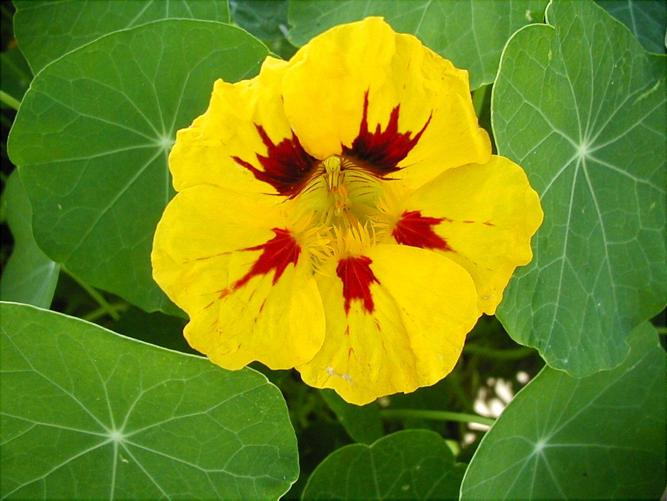
\includegraphics[width=0.7\textwidth]{images/img_train}
    \caption{Training}
  \end{subfigure}
  %
   \hfill
  \begin{subfigure}[b]{0.45\textwidth}
  \centering
    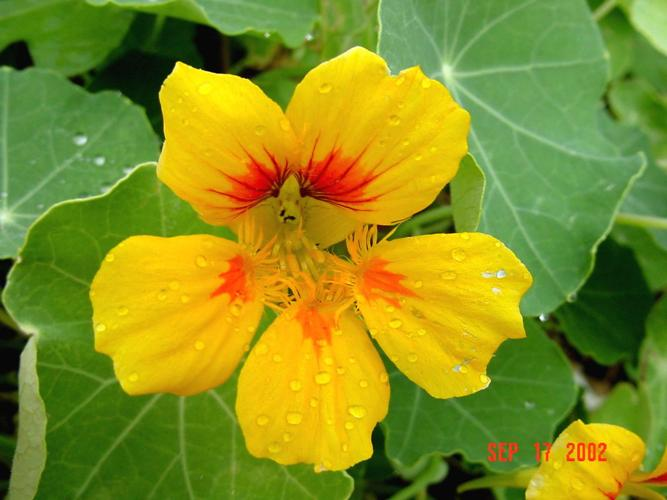
\includegraphics[width=0.7\textwidth]{images/img_test}
    \caption{Test}
  \end{subfigure}
  \caption{Confronto immagini di training e test}
  \vspace{-5mm}
  \label{fig_train_test}
\end{figure}

Gran parte delle immagini sono su sfondo neutro, generalmente foglie, questo rende probabilmente più facile per la rete concentrarsi sul fiore ignorando lo sfondo, cosa che non succede se si utilizzando pezzi di immagine.
\subsection{Esperimento 2 - Finetuning Densenet121}
La Densenet-121 \cite{huang2016densely} è un tipo di architettura considerato un'evoluzione della precedente Resnet, la rete è estremamente più profonda, aumenta il rischio di overfitting sui dati, ma dovrebbe essere in grado di ottenere risultati superiori al modello addestrato precedentemente. Le medesime tecniche di data augmentation e addestramento descritte nella sezione precedente sono utilizzate per addestrare il modello.
Anche in questo caso, come visibile in tabella \ref{t_res_densenet} Adam ottiene risultati leggermente superiori rispetto ad SGD, vi è inoltre un netto aumento del 5\% rispetto ai risultati prodotti con il modello precedente.
\subsection{Esperimento 3 - Finetuning EfficientnetB4}
Infine è stato testata una delle architetture più interessanti proposte in letteratura negli ultimi anni, la cosiddetta Efficientnet \cite{tan2019efficientnet}.
Questo tipo di architettura è stato costruito tramite tecniche automatiche di ricerca e riscalamento di architetture per reti neurali in modo tale da massimizzare contemporaneamente l'accuratezza della rete ed il numero di operazioni eseguite al secondo.
Come si vede dal grafico, la Efficientnet è in grado di ottenere performance comparabili a modelli con dieci volte il numero di parametri da addestrare.
\begin{figure}[H]

\centering
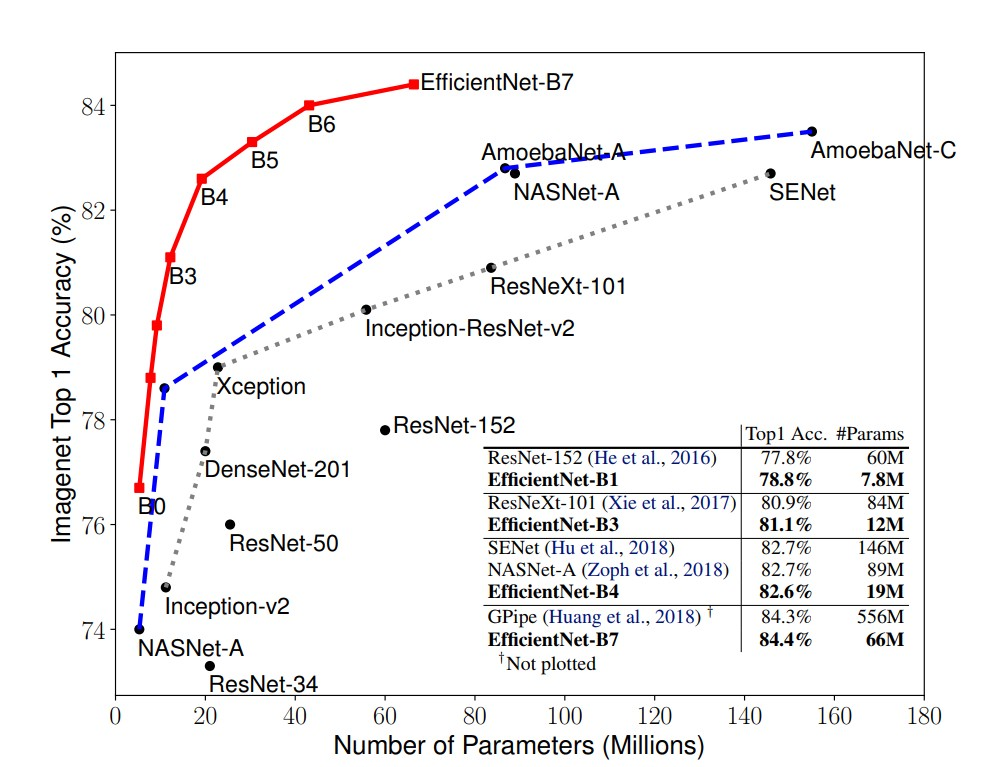
\includegraphics[width=0.6\textwidth]{images/efficientnet} 
\label{fig_efficientnet}
\caption{Confronto accuratezza rispetto al numero di parametri su imagenet}
\end{figure} 
La scelta di utilizzare il modello B4 è relativa al fatto di essere il modello migliore abbastanza leggero da essere contenuto sulla GPU utilizzata.
L'input di questa rete è costituito da immagini di dimensione 380x380, il numero di immagini per batch è stato ridotto a 8 per non incappare in overflow della memoria.
Utilizzando le stesse tecniche di addestramento già descritte si ottengono i risultati in tabella \ref{t_res_efficientnet}, anche in questo caso Adam funziona leggermente meglio di SGD e otteniamo un ulteriore aumento di accuratezza rispetto alla Densenet di circa il 5\%.

\subsection{Verifica dell'apprendimento della rete}
Per verificare su quali parti dell'immagine la rete fa maggiormente riferimento per eseguire la classificazione, utilizziamo due metodi ben noti in letteratura, le \textit{Saliency Maps} \cite{simonyan2013deep} e il grad-CAM \cite{Selvaraju_2019}.
\subsubsection{Saliency maps}
L'idea delle \textit{Saliency maps} è molto semplice, si visualizzano i gradienti di un'immagine in ingresso rispetto alla sua label calcolati sul layer di classificazione. Questa mappa dei gradienti indica quali sono le zone che più influiscono sulla classificazione corretta dell'immagine.

\begin{figure}[H]
  \begin{subfigure}[b]{0.45\textwidth}
  \centering
    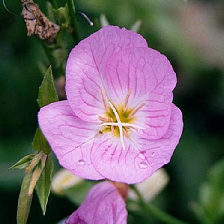
\includegraphics[width=0.7\textwidth]{images/saliency-input}
    \caption{Input}
  \end{subfigure}
  %
   \hfill
  \begin{subfigure}[b]{0.45\textwidth}
  \centering
    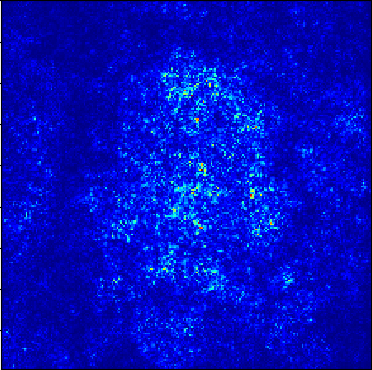
\includegraphics[width=0.7\textwidth]{images/saliency-output}
    \caption{Saliency map}
  \end{subfigure}
  \caption{Esempio di saliency map estratto dalla Desnenet121}
  \label{fig_saliency}
\end{figure}

Come si vede in figura \ref{fig_saliency} la maggior parte dei pixel che influiscono sulla classificazione è contenuta all'interno del fiore, questo è un buon indicatore della bontà del modello.
\subsubsection{grad-CAM}
Simile alle \textit{saliency maps} il grad-CAM (Class Activation Map) utilizza il gradiente dell'ultimo layer convoluzionale invece che quello dell'output, questo permette di utilizzare le informazioni spaziali perse nel passaggio da convoluzionale a completamente connesso.

\begin{figure}[H]
  \begin{subfigure}[b]{0.45\textwidth}
  \centering
    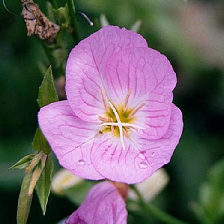
\includegraphics[width=0.7\textwidth]{images/saliency-input}
    \caption{Input}
  \end{subfigure}
  %
   \hfill
  \begin{subfigure}[b]{0.45\textwidth}
  \centering
    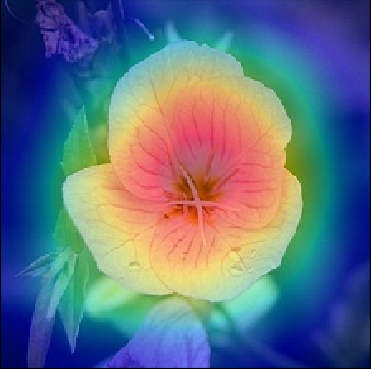
\includegraphics[width=0.7\textwidth]{images/gradcam_guided}
    \caption{Saliency map}
  \end{subfigure}
  \caption{Esempio di grad-CAM estratto dalla Desnenet121}
  \label{fig_grad_cam}
\end{figure}

In questo caso, come si vede chiaramente in figura \ref{fig_grad_cam}, è ancora più evidente come il fiore sia la componente principale nell'apprendimento della rete, si nota inoltre che l'area centrale è particolarmente discriminativa.

\section{Risultati ottenuti}
In questa sezione vengono riportari i risultati ottenuti sul test set quando si utilizzano i migliori modelli addestrati oltre che sul training anche sul validation set. I risultati sono mostrati in tabella \ref{t_res}.
\begin{table}[H]
\centering
\caption{Risultati ottenuti}
\begin{tabular}{|l|l|l|l|l|l|l|}
\hline
\textbf{architettura}   & \textbf{metodo}     & \textbf{step} & \textbf{lr range}        & \textbf{batch size} & \textbf{crop} & \textbf{test acc} \\ \hline
Resnet18       & Triangular  & 2    & {[}1e-6,5e-4{]} & 64         & No   & 0.9187   \\ \hline
Densenet121    & Triangular  & 4    & {[}1e-5,1e-3{]} & 64         & No   & 0.9455   \\ \hline
EfficientnetB4 & Triangular2 & 4    & {[}1e-5,1e-3{]} & 8          & No   & \textbf{0.9719}   \\ \hline
\end{tabular}
\label{t_res}
\end{table}

Viene poi mostrato il confronto con gli algoritmi proposti in letteratura, alcuni di questi (\cite{Nilsback08}, \cite{yaqub}, \cite{XIE2017118}) fanno uso anche dei fiori segmentati per la classificazione.
\begin{table}[H]
\centering
\caption{Confronto con risultati in letteratura}
\begin{tabular}{|l|l|}
\hline
\textbf{metodo}                                           & \textbf{test acc} \\ \hline
EfficientnetB4                                            & \textbf{0.9719}           \\ \hline
Nilsback and Zisserman \cite{Nilsback08} & 0.7280            \\ \hline
Yaqub et. al \cite{yaqub}                & 0.9710            \\ \hline
CNN-RI-Deep \cite{Xie2016TowardsRI}      & 0.9401            \\ \hline
Zheng et al. \cite{zheng2016good}        & 0.9560            \\ \hline
Inception-v3 \cite{7984661}              & 0.9400            \\ \hline
LG-CNN \cite{XIE2017118}                 & 0.9660            \\ \hline
\end{tabular}
\label{t_conf}
\end{table}
\section{Discussione}
Gli obiettivi discussi inizialmente sono stati raggiunti, grazie ala combinazione di moderne architetture e tecniche di addestramento si è in grado di ottenere risultati comparabili a tecniche molto più sofisticate sviluppate da ricercatori esperti. Ci si aspettava dei risultati migliori per quanto riguarda l'addestramento delle reti su ritagli di immagini, questo tipo di modelli potrebbero funzionare meglio di quelli addestrati sulle intere immagini se testati su un dataset più complesso. Per ottenere un ulteriore aumento delle performance potrebbe essere possibile integrare le segmentazioni delle immagini come canale di input per la rete, questo dovrebbe migliorare sicuramente le performance sul dataset in oggetto, ma richiederebbe la conoscenza di queste immagini anche nel caso si volesse testare la rete su dati nuovi, limitandone l'utilizzo reale.
\newpage
\section{Conclusioni}
Classificare un dataset con molte classi simili tra di loro è ormai possibile grazie agli incredibili avanzamenti in materia di ottimizzazione e architetture di reti neurali. Come mostrato in questo lavoro il semplice utilizzo di tecniche moderne permette di ottenere performance estremamente elevate, senza dover necessariamente andare ad inventare architetture o algoritmi molto più complessi. In un mondo sempre più indirizzato verso l'autoML la scelta di utilizzare tecniche di ottimizzazione e architetture automatizzate sembra la più sensata, nonostante ciò l'intervento umano richiesto è comunque ancora parecchio evidente. Come già citato in precedenza ci sono alcune tecniche testabili in futuro per aumentare ulteriormente le performance, sarebbe inoltre interessante costruire un nuovo dataset con le stesse classi, ma molto più grande e complesso, per verificare ulteriormente quali tecniche funzionino realmente meglio. Come si è visto anche una semplice Resnet18, architettura proposta cinque anni fa e non particolarmente profonda ottiene delle performance superiori al 90\%. Il dataset in oggetto, proposto ormai nel lontano 2008 è quasi vicino al punto in cui una rete neurale è perfettamente in grado di classificarlo!

\section*{Ringraziamenti}
Gli autori ringraziano il supporto del Consortium GARR per aver permesso l'utilizzo di una Nvidia Tesla V100 su cui sono stati eseguiti tutti gli esperimenti.
\newpage
\bibliographystyle{IEEEtran}
\bibliography{references}

\newpage
\appendix
\section{Risultati sperimentali}
\subsection{Resnet18}
\begin{table}[H]
\centering
\caption{Dettagli addestramento}
\begin{tabular}{|l|l|l|l|l|}
\hline
\textbf{ott} & \textbf{range lr} & \textbf{epoche} & \textbf{batch size} & \textbf{tempo training medio} \\ \hline
SGD          & [1e-5, 1e-3]         & 50              & 64                  & 300s                          \\ \hline
Adam         & [1e-6, 5e-4]         & 50              & 64                  & 300s                          \\ \hline
\end{tabular}
\end{table}
\begin{table}[H]
\centering
\caption{Risultati finetuning resnet18}
\begin{adjustbox}{width=1\textwidth}
\begin{tabular}{|l|l|l|l|l|l||l|l|l|l|l|l|}
\hline
\textbf{tipo} & \textbf{ott} & \textbf{crop} & \textbf{metodo} & \textbf{step} & \textbf{test acc} & \textbf{tipo} & \textbf{ott} & \textbf{crop} & \textbf{method} & \textbf{step} & \textbf{test acc} \\ \hline
acc           & sgd          & base          & triangular      & 2             & 0.7627            & acc           & adam         & base          & triangular      & 2             & 0.8619   \\ \hline
loss          & sgd          & base          & triangular      & 2             & 0.7627            & loss          & adam         & No          & triangular      & 2             & \textbf{0.8632}            \\ \hline
acc           & sgd          & No          & triangular      & 4             & 0.7528            & acc           & adam         & No          & triangular      & 4             & 0.8554            \\ \hline
loss          & sgd          & No          & triangular      & 4             & 0.7583            & loss          & adam         & No          & triangular      & 4             & 0.8578            \\ \hline
acc           & sgd          & No          & triangular      & 6             & 0.7436            & acc           & adam         & No          & triangular      & 6             & 0.8510            \\ \hline
loss          & sgd          & No          & triangular      & 6             & 0.7436            & loss          & adam         & No          & triangular      & 6             & 0.8537            \\ \hline
acc           & sgd          & No          & triangular      & 8             & 0.7604            & acc           & adam         & No          & triangular      & 8             & 0.8565            \\ \hline
loss          & sgd          & No          & triangular      & 8             & 0.7604            & loss          & adam         & No          & triangular      & 8             & 0.8603            \\ \hline
acc           & sgd          & No          & triangular2     & 2             & 0.2663            & acc           & adam         & No          & triangular2     & 2             & 0.8248            \\ \hline
loss          & sgd          & No          & triangular2     & 2             & 0.2663            & loss          & adam         & No          & triangular2     & 2             & 0.8246            \\ \hline
acc           & sgd          & No          & triangular2     & 4             & 0.5077            & acc           & adam         & No          & triangular2     & 4             & 0.8388            \\ \hline
loss          & sgd          & No          & triangular2     & 4             & 0.5077            & loss          & adam         & No          & triangular2     & 4             & 0.8485            \\ \hline
acc           & sgd          & No          & triangular2     & 6             & 0.6111            & acc           & adam         & No          & triangular2     & 6             & 0.8414            \\ \hline
loss          & sgd          & No          & triangular2     & 6             & 0.6111            & loss          & adam         & No          & triangular2     & 6             & 0.8497            \\ \hline
acc           & sgd          & No          & triangular2     & 8             & 0.6638            & acc           & adam         & No          & triangular2     & 8             & 0.8472            \\ \hline
loss          & sgd          & No          & triangular2     & 8             & 0.6640            & loss          & adam         & No          & triangular2     & 8             & 0.8484            \\ \hline
acc           & sgd          & random        & triangular      & 2             & 0.7015            & acc           & adam         & random        & triangular      & 2             & 0.8388            \\ \hline
loss          & sgd          & random        & triangular      & 2             & 0.7036            & loss          & adam         & random        & triangular      & 2             & 0.8412            \\ \hline
acc           & sgd          & random        & triangular      & 4             & 0.7127            & acc           & adam         & random        & triangular      & 4             & 0.8266            \\ \hline
loss          & sgd          & random        & triangular      & 4             & 0.7127            & loss          & adam         & random        & triangular      & 4             & 0.8256            \\ \hline
acc           & sgd          & random        & triangular      & 6             & 0.7017            & acc           & adam         & random        & triangular      & 6             & 0.8326            \\ \hline
loss          & sgd          & random        & triangular      & 6             & 0.7017            & loss          & adam         & random        & triangular      & 6             & 0.8376            \\ \hline
acc           & sgd          & random        & triangular      & 8             & 0.7150            & acc           & adam         & random        & triangular      & 8             & 0.8248            \\ \hline
loss          & sgd          & random        & triangular      & 8             & 0.7150            & loss          & adam         & random        & triangular      & 8             & 0.8274            \\ \hline
acc           & sgd          & random        & triangular2     & 2             & 0.2263            & acc           & adam         & random        & triangular2     & 2             & 0.7906            \\ \hline
loss          & sgd          & random        & triangular2     & 2             & 0.2267            & loss          & adam         & random        & triangular2     & 2             & 0.7906            \\ \hline
acc           & sgd          & random        & triangular2     & 4             & 0.4338            & acc           & adam         & random        & triangular2     & 4             & 0.8243            \\ \hline
loss          & sgd          & random        & triangular2     & 4             & 0.4351            & loss          & adam         & random        & triangular2     & 4             & 0.8256            \\ \hline
acc           & sgd          & random        & triangular2     & 6             & 0.5594            & acc           & adam         & random        & triangular2     & 6             & 0.8268            \\ \hline
loss          & sgd          & random        & triangular2     & 6             & 0.5607            & loss          & adam         & random        & triangular2     & 6             & 0.8272            \\ \hline
acc           & sgd          & random        & triangular2     & 8             & 0.6152            & acc           & adam         & random        & triangular2     & 8             & 0.8323            \\ \hline
loss          & sgd          & random        & triangular2     & 8             & 0.6158            & loss          & adam         & random        & triangular2     & 8             & 0.8297            \\ \hline
\end{tabular}
\end{adjustbox}
\label{t_res_resnet}
\end{table}

\subsection{Densenet121}

\begin{table}[H]
\centering
\caption{Dettagli addestramento}
\begin{tabular}{|l|l|l|l|l|}
\hline
\textbf{ott} & \textbf{range lr} & \textbf{epoche} & \textbf{batch size} & \textbf{tempo training medio} \\ \hline
SGD          & [1e-5, 1e-2]         & 50              & 64                  & 450s                          \\ \hline
Adam         & [1e-5, 1e-3]        & 50              & 64                  & 450s                          \\ \hline
\end{tabular}
\end{table}
\begin{table}[H]
\centering
\caption{Risultati finetuning Densenet121}
\begin{adjustbox}{width=1\textwidth}
\begin{tabular}{|l|l|l|l|l|l||l|l|l|l|l|l|}
\hline
\textbf{tipo} & \textbf{ott} & \textbf{crop} & \textbf{metodo} & \textbf{step} & \textbf{test acc} & \textbf{tipo} & \textbf{ott} & \textbf{crop} & \textbf{metodod} & \textbf{step} & \textbf{test acc} \\ \hline
acc           & sgd          & No          & triangular       & 2             & 0.8934            & loss          & sgd          & random        & triangular2      & 8             & 0.8866            \\ \hline
loss          & sgd          & No          & triangular       & 2             & 0.8955            & acc           & adam         & No          & triangular       & 2             & 0.9094            \\ \hline
acc           & sgd          & No          & triangular       & 4             & 0.8910            & loss          & adam         & No          & triangular       & 2             & 0.9094            \\ \hline
loss          & sgd          & No          & triangular       & 4             & 0.8939            & acc           & adam         & No          & triangular       & 4             & \textbf{0.9108}   \\ \hline
acc           & sgd          & No          & triangular       & 6             & 0.9009            & loss          & adam         & No          & triangular       & 4             & 0.9103            \\ \hline
loss          & sgd          & No          & triangular       & 6             & 0.9019            & acc           & adam         & No          & triangular       & 6             & 0.9056            \\ \hline
acc           & sgd          & No          & triangular       & 8             & 0.8981            & loss          & adam         & No          & triangular       & 6             & 0.9081            \\ \hline
loss          & sgd          & No          & triangular       & 8             & 0.9020            & acc           & adam         & No          & triangular       & 8             & 0.9063            \\ \hline
acc           & sgd          & No          & triangular2      & 2             & 0.8765            & loss          & adam         & No          & triangular       & 8             & 0.9063            \\ \hline
loss          & sgd          & No          & triangular2      & 2             & 0.8733            & acc           & adam         & No          & triangular2      & 2             & 0.8973            \\ \hline
acc           & sgd          & No          & triangular2      & 4             & 0.8885            & loss          & adam         & No          & triangular2      & 2             & 0.8975            \\ \hline
loss          & sgd          & No          & triangular2      & 4             & 0.8884            & acc           & adam         & No          & triangular2      & 4             & 0.9073            \\ \hline
acc           & sgd          & No          & triangular2      & 6             & 0.8957            & loss          & adam         & No          & triangular2      & 4             & 0.9074            \\ \hline
loss          & sgd          & No          & triangular2      & 6             & 0.8786            & acc           & adam         & No          & triangular2      & 6             & 0.9076            \\ \hline
acc           & sgd          & No          & triangular2      & 8             & 0.8965            & loss          & adam         & No          & triangular2      & 6             & 0.9097            \\ \hline
loss          & sgd          & No          & triangular2      & 8             & 0.8967            & acc           & adam         & No          & triangular2      & 8             & 0.9029            \\ \hline
acc           & sgd          & random        & triangular       & 2             & 0.8816            & loss          & adam         & No          & triangular2      & 8             & 0.9056            \\ \hline
loss          & sgd          & random        & triangular       & 2             & 0.8827            & acc           & adam         & random        & triangular       & 2             & 0.8921            \\ \hline
acc           & sgd          & random        & triangular       & 4             & 0.8874            & loss          & adam         & random        & triangular       & 2             & 0.8918            \\ \hline
loss          & sgd          & random        & triangular       & 4             & 0.8874            & acc           & adam         & random        & triangular       & 4             & 0.9030            \\ \hline
acc           & sgd          & random        & triangular       & 6             & 0.8835            & loss          & adam         & random        & triangular       & 4             & 0.9030            \\ \hline
loss          & sgd          & random        & triangular       & 6             & 0.8851            & acc           & adam         & random        & triangular       & 6             & 0.8986            \\ \hline
acc           & sgd          & random        & triangular       & 8             & 0.8816            & loss          & adam         & random        & triangular       & 6             & 0.8986            \\ \hline
loss          & sgd          & random        & triangular       & 8             & 0.8876            & acc           & adam         & random        & triangular       & 8             & 0.8928            \\ \hline
acc           & sgd          & random        & triangular2      & 2             & 0.8474            & loss          & adam         & random        & triangular       & 8             & 0.8951            \\ \hline
loss          & sgd          & random        & triangular2      & 2             & 0.8474            & acc           & adam         & random        & triangular2      & 2             & 0.8804            \\ \hline
acc           & sgd          & random        & triangular2      & 4             & 0.8770            & loss          & adam         & random        & triangular2      & 2             & 0.8817            \\ \hline
loss          & sgd          & random        & triangular2      & 4             & 0.8780            & acc           & adam         & random        & triangular2      & 4             & 0.8881            \\ \hline
acc           & sgd          & random        & triangular2      & 6             & 0.8833            & loss          & adam         & random        & triangular2      & 4             & 0.8879            \\ \hline
loss          & sgd          & random        & triangular2      & 6             & 0.8858            & acc           & adam         & random        & triangular2      & 6             & 0.8990            \\ \hline
acc           & sgd          & random        & triangular2      & 8             & 0.8814            & loss          & adam         & random        & triangular2      & 6             & 0.8991            \\ \hline
loss          & sgd          & random        & triangular2      & 8             & 0.8837            & acc           & adam         & random        & triangular2      & 8             & 0.8894            \\ \hline
\end{tabular}
\end{adjustbox}
\label{t_res_densenet}
\end{table}

\subsection{EfficientnetB4}

\begin{table}[H]
\centering
\caption{Dettagli addestramento}
\begin{tabular}{|l|l|l|l|l|}
\hline
\textbf{ott} & \textbf{range lr} & \textbf{epoche} & \textbf{batch size} & \textbf{tempo training medio} \\ \hline
SGD          & {[}1e-5, 1e-3{]}   & 50              & 8                   & 2000s                         \\ \hline
Adam         & {[}1e-5, 1e-3{]}  & 50              & 68                  & 2000s                         \\ \hline
\end{tabular}
\end{table}
\begin{table}[H]
\centering
\caption{Risultati finetuning EfficientnetB4}
\begin{adjustbox}{width=1\textwidth}
\begin{tabular}{|l|l|l|l|l|l||l|l|l|l|l|l|}
\hline
\textbf{tipo} & \textbf{ott} & \textbf{crop} & \textbf{metodo} & \textbf{step} & \textbf{test acc} & \textbf{tipo} & \textbf{ott} & \textbf{crop} & \textbf{metodo} & \textbf{step} & \textbf{test acc} \\ \hline
acc           & sgd          & No          & triangular      & 2             & 0.9198            & acc           & adam         & No          & triangular      & 2             & 0.9105            \\ \hline
loss          & sgd          & No          & triangular      & 2             & 0.9198            & loss          & adam         & No          & triangular      & 2             & 0.9105            \\ \hline
acc           & sgd          & No          & triangular      & 4             & 0.9173            & acc           & adam         & No          & triangular      & 4             & 0.9386            \\ \hline
loss          & sgd          & No          & triangular      & 4             & 0.9173            & loss          & adam         & No          & triangular      & 4             & 0.9386            \\ \hline
acc           & sgd          & No          & triangular      & 6             & 0.9164            & acc           & adam         & No          & triangular      & 6             & 0.9261            \\ \hline
loss          & sgd          & No          & triangular      & 6             & 0.9183            & loss          & adam         & No          & triangular      & 6             & 0.9261            \\ \hline
acc           & sgd          & No          & triangular      & 8             & 0.9164            & acc           & adam         & No          & triangular      & 8             & 0.9302            \\ \hline
loss          & sgd          & No          & triangular      & 8             & 0.9164            & loss          & adam         & No          & triangular      & 8             & 0.9329            \\ \hline
acc           & sgd          & No          & triangular2     & 2             & 0.5316            & acc           & adam         & No          & triangular2     & 2             & 0.9492            \\ \hline
loss          & sgd          & No          & triangular2     & 2             & 0.5394            & loss          & adam         & No          & triangular2     & 2             & 0.9490            \\ \hline
acc           & sgd          & No          & triangular2     & 4             & 0.7371            & acc           & adam         & No          & triangular2     & 4             & \textbf{0.9567}   \\ \hline
loss          & sgd          & No          & triangular2     & 4             & 0.7375            & loss          & adam         & No          & triangular2     & 4             & 0.9559            \\ \hline
acc           & sgd          & No          & triangular2     & 6             & 0.8211            & acc           & adam         & No          & triangular2     & 6             & 0.9411            \\ \hline
loss          & sgd          & No          & triangular2     & 6             & 0.8250            & loss          & adam         & No          & triangular2     & 6             & 0.9447            \\ \hline
acc           & sgd          & No          & triangular2     & 8             & 0.8692            & acc           & adam         & No          & triangular2     & 8             & 0.9393            \\ \hline
loss          & sgd          & No          & triangular2     & 8             & 0.8697            & loss          & adam         & No          & triangular2     & 8             & 0.9393            \\ \hline
acc           & sgd          & random        & triangular      & 2             & 0.9092            & acc           & adam         & random        & triangular      & 2             & 0.8923            \\ \hline
loss          & sgd          & random        & triangular      & 2             & 0.9092            & loss          & adam         & random        & triangular      & 2             & 0.8923            \\ \hline
acc           & sgd          & random        & triangular      & 4             & 0.9116            & acc           & adam         & random        & triangular      & 4             & 0.9141            \\ \hline
loss          & sgd          & random        & triangular      & 4             & 0.9116            & loss          & adam         & random        & triangular      & 4             & 0.9141            \\ \hline
acc           & sgd          & random        & triangular      & 6             & 0.9079            & acc           & adam         & random        & triangular      & 6             & 0.9128            \\ \hline
loss          & sgd          & random        & triangular      & 6             & 0.9121            & loss          & adam         & random        & triangular      & 6             & 0.9128            \\ \hline
acc           & sgd          & random        & triangular      & 8             & 0.9094            & acc           & adam         & random        & triangular      & 8             & 0.9168            \\ \hline
loss          & sgd          & random        & triangular      & 8             & 0.9110            & loss          & adam         & random        & triangular      & 8             & 0.9208            \\ \hline
acc           & sgd          & random        & triangular2     & 2             & 0.4844            & acc           & adam         & random        & triangular2     & 2             & 0.9386            \\ \hline
loss          & sgd          & random        & triangular2     & 2             & 0.4815            & loss          & adam         & random        & triangular2     & 2             & 0.9395            \\ \hline
acc           & sgd          & random        & triangular2     & 4             & 0.7119            & acc           & adam         & random        & triangular2     & 4             & 0.9355            \\ \hline
loss          & sgd          & random        & triangular2     & 4             & 0.7118            & loss          & adam         & random        & triangular2     & 4             & 0.9370            \\ \hline
acc           & sgd          & random        & triangular2     & 6             & 0.7978            & acc           & adam         & random        & triangular2     & 6             & 0.9305            \\ \hline
loss          & sgd          & random        & triangular2     & 6             & 0.7978            & loss          & adam         & random        & triangular2     & 6             & 0.9331            \\ \hline
acc           & sgd          & random        & triangular2     & 8             & 0.8492            & acc           & adam         & random        & triangular2     & 8             & 0.9284            \\ \hline
loss          & sgd          & random        & triangular2     & 8             & 0.8502            & loss          & adam         & random        & triangular2     & 8             & 0.9284            \\ \hline
\end{tabular}
\end{adjustbox}
\label{t_res_efficientnet}
\end{table}
\end{document}
